% HADES 2.0 manuscript. Every number comes from tables/numbers.tex and tables/*.tex, which
% scripts/paper/make_figures.py generates from results/processed/paper_numbers.json
% (scripts/paper/recompute_headlines.py, recomputed from results/raw/). Do not type numbers by hand.
\documentclass[conference]{IEEEtran}
\usepackage{amsmath,amssymb}
\usepackage{booktabs}
\usepackage{graphicx}
\usepackage{cite}
\usepackage{url}
\usepackage{xcolor}
\usepackage[hidelinks]{hyperref}
% generated by scripts/paper/make_figures.py; do not edit
\newcommand{\numUR}{0.27}
\newcommand{\numURlo}{0.23}
\newcommand{\numURhi}{0.30}
\newcommand{\numUJ}{0.22}
\newcommand{\numUJlo}{0.19}
\newcommand{\numUJhi}{0.26}
\newcommand{\numURmis}{0.05}
\newcommand{\numURmislo}{0.01}
\newcommand{\numURmishi}{0.10}
\newcommand{\numUJth}{-0.03}
\newcommand{\numUJthlo}{-0.09}
\newcommand{\numUJthhi}{0.03}
\newcommand{\numLJ}{0.11}
\newcommand{\numLJlo}{0.06}
\newcommand{\numLJhi}{0.17}
\newcommand{\numLC}{0.02}
\newcommand{\numLClo}{-0.02}
\newcommand{\numLChi}{0.06}
\newcommand{\numLJmis}{-0.05}
\newcommand{\numLJmislo}{-0.13}
\newcommand{\numLJmishi}{0.02}
\newcommand{\numLJcov}{0.49}
\newcommand{\numLJcovlo}{0.41}
\newcommand{\numLJcovhi}{0.56}
\newcommand{\numTR}{-0.19}
\newcommand{\numTRlo}{-0.28}
\newcommand{\numTRhi}{-0.10}
\newcommand{\numTM}{-0.02}
\newcommand{\numTMlo}{-0.08}
\newcommand{\numTMhi}{0.04}
\newcommand{\numVnA}{100}
\newcommand{\numVattA}{50}
\newcommand{\numVspA}{19}
\newcommand{\numVoneA}{0.040}
\newcommand{\numVoneloA}{-0.041}
\newcommand{\numVonehiA}{0.119}
\newcommand{\numVRA}{0.09}
\newcommand{\numVRloA}{-0.18}
\newcommand{\numVRhiA}{0.30}
\newcommand{\numVJA}{-0.56}
\newcommand{\numVJloA}{-1.44}
\newcommand{\numVJhiA}{-0.12}
\newcommand{\numVnB}{98}
\newcommand{\numVattB}{49}
\newcommand{\numVspB}{15}
\newcommand{\numVoneB}{-0.083}
\newcommand{\numVoneloB}{-0.172}
\newcommand{\numVonehiB}{0.004}
\newcommand{\numVRB}{0.01}
\newcommand{\numVRloB}{-0.16}
\newcommand{\numVRhiB}{0.15}
\newcommand{\numVJB}{-0.03}
\newcommand{\numVJloB}{-0.20}
\newcommand{\numVJhiB}{0.11}
\newcommand{\numVndev}{76}
\newcommand{\numVfailh}{0.355}
\newcommand{\numVfails}{0.674}
\newcommand{\numnWL}{140}
\newcommand{\numnEL}{201{,}600}
\newcommand{\numnWT}{400}
\newcommand{\numnET}{499{,}200}
\newcommand{\numnWU}{400}
\newcommand{\numnEU}{537{,}600}

\makeatletter\let\tabinput\@@input\makeatother % primitive input, so \bottomrule may follow inside tabular
\newcommand{\pol}[1]{\textsf{#1}}

\begin{document}

\title{What Helps When Telemetry Lies?\\Four Pre-Registered Tests of Evidence Acquisition\\under Source Compromise}

\author{\IEEEauthorblockN{Aakash G.S.}
\IEEEauthorblockA{gsaakash@outlook.com}}

\maketitle

\begin{abstract}
A threat hunter with a fixed budget must choose which telemetry sources to read, knowing that some of them may be
controlled by the attacker. Acquisition rules for this setting are rarely compared at equal spend, against attackers
they were not designed for, with the comparison fixed before the data exist. We run four pre-registered experiments,
each changing one part of a Bayesian acquisition policy while the shared posterior, the terminal decision, the horizon
and the spend stay fixed. Three run in a simulator over procedurally generated worlds (\numnEL, \numnET\ and \numnEU\
policy-episodes) and one on a public industrial-control dataset. Two ideas fail their gates. Valuing integrity probes by
their decision consequences adds nothing over hypothesis information under the same model (relative regret reduction
$\numLC$, 95\% CI [$\numLClo$, $\numLChi$]). Randomised and minimax acquisition do not beat a non-robust policy on a
held-out attacker ($\numTR$ and $\numTM$). One passes every gate: in simulation, scoring evidence by hypothesis
information under a joint posterior over the hypothesis and every source's compromise state reduces regret on a
held-out attacker by $\numUR$ [$\numURlo$, $\numURhi$] relative to reliability-weighted information gain and by $\numUJ$
[$\numUJlo$, $\numUJhi$] relative to joint-state information gain. The held-out attacker lies partly in the direction the
defender's model assumes. The gain is large against cover-up and decoy attackers, small against misattribution, and
against an attacker that adapts to the defender's queries it survives only relative to reliability weighting; there
random acquisition is best. A replication on the HAI dataset was invalid by its own pre-registered check, because the
mapped evidence did not beat a decision from the prior alone, so the positive result is simulator-only.
\end{abstract}

\begin{IEEEkeywords}
threat hunting, adversarial telemetry, active hypothesis testing, value of information, pre-registration, negative results
\end{IEEEkeywords}

% ---------------------------------------------------------------------------
\section{Introduction}

Attackers tamper with the evidence defenders rely on. Log deletion, forwarder sabotage and sensor spoofing are
catalogued techniques (MITRE ATT\&CK T1562, ``Impair Defenses'' \cite{attackt1562}), and holding a process variable at a
stale value is a standard attack on industrial control systems \cite{shin2020hai,urbina2016}. A hunter who investigates
an alert under a budget therefore faces two coupled questions: which source to read next, and how far to believe it.

Each piece of this problem has a long history. Choosing the next measurement by expected entropy reduction over a
joint fault model goes back to the General Diagnostic Engine \cite{dekleer1987}; decision-theoretic troubleshooting
values tests by their effect on the repair decision \cite{heckerman1995}; active sequential hypothesis testing gives
asymptotically optimal sensing rules \cite{naghshvar2013}; and Byzantine detection studies inference when some sensors
lie \cite{marano2009,soltanmohammadi2012,li2021byz}. Recent work combines a belief over compromised sensors with active
probing in cyber-physical control \cite{andersson2026} and learns cost-aware sensor scheduling with a Byzantine
detector \cite{zhong2025}.

What is missing is a controlled answer to a practical question: \emph{which part of such a policy actually reduces
decision errors when sources lie?} A new policy usually differs from its baseline in several ways at once (belief model,
objective, look-ahead, cost handling), is evaluated against the attacker its model assumes, and is compared at unequal
spend. Any of these can manufacture an apparent gain.

We address this with an ablation discipline rather than a new method. Every policy in this paper shares the same exact
posterior, the same Bayes terminal decision and exactly the same spend; policies differ only in how they score the next
action. Each experiment changes one part, names its comparators, fixes a practical threshold (a 10\% relative cut in
regret) and its gates in a committed protocol, and is tested on an attacker written after the policies were frozen.

\textbf{Contributions.}
\begin{enumerate}
\item A spend-matched, pre-registered testbed for evidence acquisition under source compromise: procedurally generated
worlds, five attacker families of which three were each held out from one experiment's design, and frozen gate code
(Sec.~\ref{sec:setup}).
\item Two pre-registered negative results. Valuing source-integrity probes by their decision consequences adds no
robust gain over hypothesis information under the same joint model, and neither randomised nor minimax acquisition
beats the non-robust comparator on a held-out attacker (Sec.~\ref{sec:neg}).
\item One scoped positive result. At equal objective, horizon and cost handling, replacing a reliability-weighted
look-ahead model with the joint model over hypothesis and source states reduces regret by $\numUR$ on a held-out
attacker, and replacing the joint-entropy objective with hypothesis entropy reduces it by $\numUJ$. We report where
both gains shrink or vanish (Sec.~\ref{sec:pos}).
\item A real-data attempt on the HAI industrial-control dataset that failed its own validity check, with the reasons, so
that the positive result is reported as simulator-only (Sec.~\ref{sec:hai}).
\end{enumerate}

\textbf{Scope.} All positive evidence comes from one simulator family and one world distribution, with policies and
attackers written by the same author. We do not claim the joint belief model as new; it is classical
\cite{dekleer1987,heckerman1995,soltanmohammadi2012}. The contribution is controlled evidence about which part
matters, and where it stops mattering.

% ---------------------------------------------------------------------------
\section{Related Work}

\textbf{Diagnosis and troubleshooting.} GDE selects measurements by minimum expected entropy over component states
\cite{dekleer1987}; Bayesian-network test selection does the same at scale \cite{zheng2005}; decision-theoretic
troubleshooting values tests by their effect on the repair decision \cite{heckerman1995}. Faults there are not
strategic, and observations of healthy components are trusted. Our joint-state objective $J$ is the GDE criterion and
our decision-value probe $P$ follows the troubleshooting criterion.

\textbf{Sensing with adversarial sources.} Byzantine detection studies fusion when a fraction of sensors lie, through
error exponents and game equilibria with all sensors observed \cite{marano2009,li2021byz}. Soltanmohammadi et al.\
infer node identity jointly with the hypothesis by EM \cite{soltanmohammadi2012}, the closest inference-side match to
our belief model, but without a choice of which source to read. Andersson and D\'an maintain a Bayesian network over
sensor attack states and choose a control input that maximises a KL divergence between attack hypotheses, with the goal
of control recovery \cite{andersson2026}. Zhong et al.\ learn sensor scheduling with probing costs and a separate
Byzantine detector \cite{zhong2025}. MATE estimates per-agent trust as a hidden state for fusion \cite{hallyburton2025}.
In industrial control, residual-based detectors and their limits against stealthy attacks are well studied
\cite{urbina2016}; our HAI probe is a simple instance. None of these ablates the belief model against the objective at
equal spend, or evaluates on attackers written after the policy.

\textbf{Active learning with unreliable oracles.} Proactive learning selects among imperfect, cost-varying oracles
\cite{donmez2008}; cost-aware active learning divides information by cost \cite{settles2008,settles2009}. Oracle noise
there is not strategic.

\textbf{Security operations.} POMDP and optimal-stopping formulations plan sensing, prevention and response under noisy
alerts \cite{mccarthy2016,miehling2018,hammar2021}, but treat alert noise as non-strategic. Forward-secure and
tamper-evident logging \cite{schneier1999,custos2020} protect the integrity a probe would check; provenance triage
\cite{nodoze2019} and hunting under anti-forensics \cite{hunteragent2026} motivate our compromised-source model. These
works do not choose evidence decision-theoretically under source compromise.

% ---------------------------------------------------------------------------
\section{Problem and Policies}\label{sec:model}

\textbf{Operational picture.} A hunter triages an alert on a host. The sources are the telemetry a SOC would pull: EDR,
Sysmon, authentication logs, DNS, proxy, NetFlow, cloud audit logs, mail gateway. A query pulls evidence from one
source; it can be forged if the attacker controls that source's sensor or forwarder. A probe is an integrity check on
one source: inject a canary event and verify it arrives intact, check the forwarder's heartbeat or hash chain, or
cross-check the source against an independent sensor. The final decision is to dismiss the alert, contain the host or
block egress.

\textbf{State.} A hidden hypothesis $H\in\{\text{benign},\text{intrusion}_1,\text{intrusion}_2\}$ and, for each of $K$
sources, a state $S_q\in\{\text{healthy},\text{degraded},\text{compromised}\}$. A healthy source reports the true
hypothesis with probability $\mathrm{acc}_q$; a degraded one reports uniformly; a compromised one, in the defender's
model, forges its report with probability 0.9: a cover-up (``benign'') under an intrusion, a false flag under benign. A
probe returns PASS or FAIL with state-dependent rates. Compromise is less likely under benign activity:
$P(S_q{=}C\mid\text{benign})=\kappa\,P(S_q{=}C\mid\text{intrusion})$. Sources are conditionally independent given $(H,S)$,
which ignores shared failure modes such as one host agent feeding several sources (Sec.~\ref{sec:threats}).

\textbf{Decision and regret.} After the budget is spent, the defender takes $D^*=\arg\max_D\mathbb{E}[U(D,H)\mid E]$:
0 if correct, $-L_{\text{miss}}$ for dismissing an intrusion, $-0.5L_{\text{miss}}$ for the wrong containment, $-1$ for
a false alarm. Regret is $U(D^*(H),H)-U(D,H)$ divided by $L_{\text{miss}}$, so it lies in $[0,1]$.

\textbf{Shared machinery.} Every policy sees the same exact posterior $P(H,S_1,\dots,S_K\mid E)$, and the simulator, not
the policy, applies the same Bayes decision. Costs are integers with a fixed budget, and every policy must act while it
can afford an action, so every policy spends exactly the budget in every episode (checked in every run). Policies never
see the true hypothesis, source states or attacker identity; leakage tests enforce this.

\textbf{Policies differ only in scoring.} A score has three parts: the \emph{model} used for look-ahead, the
\emph{objective} credited per outcome, and the \emph{horizon}. With horizon 2 and cost-awareness,
$\text{score}(a)=\max\big(V_1(a)/c_a,\ \max_b V_2(a,b)/(c_a+c_b)\big)$. The four policies that matter are:
\begin{itemize}
\item $R$ (\pol{P3\_RHAT\_COST\_LA2}): reliability-weighted look-ahead. A query of $q$ is scored as
$\hat r_q\,p_{\text{nom}}+(1-\hat r_q)\,\text{uniform}$, with $\hat r_q$ the current posterior probability that $q$ is
healthy. Objective: entropy reduction of $H$.
\item $C$ (\pol{P\_JOINT\_HEIG\_COST}): exact joint look-ahead; objective: entropy reduction of $H$.
\item $J$ (\pol{P\_JOINT\_EIG\_COST}): exact joint look-ahead; objective: entropy reduction of $(H,S)$, the GDE criterion.
\item $P$ (\pol{P\_PROBE}): exact joint look-ahead; objective: expected gain in the Bayes-decision utility (value of
information), falling back to $H$-information on VoI plateaus.
\end{itemize}
All four use horizon 2 and divide by cost. $C$ and $J$ differ only in the objective. $C$ and $R$ differ only in the
look-ahead model, but that model difference is a package of four choices: $R$ treats a compromised source as symmetric
noise rather than as a cover-up forger; it drops the coupling $\kappa$ between $H$ and $S$; in its look-ahead a query
updates $H$ but not the queried source's state, so repeated reads of one source count as independent; and it credits a
probe with no immediate $H$-information. Our experiments do not separate these four. References include random
acquisition, nominal EIG that ignores cost and compromise (\pol{P3\_NOM}), and, in E2, two robust variants of $J$.

% ---------------------------------------------------------------------------
\section{Experimental Setup}\label{sec:setup}

\textbf{Worlds.} Each unit of analysis is a world drawn from a frozen distribution: $K\sim U\{5..8\}$ sources;
$P(\text{benign})\sim U(0.30,0.80)$, the rest split evenly; source accuracy $U(0.45,0.95)$; query cost $U\{1..4\}$ with
one source forced to 1; probe cost $\max(1,\mathrm{round}(r c_q))$ with $r\sim$ log-$U(0.25,2)$; compromise prior
$\pi\sim U(0.02,0.40)$ with per-source jitter $U(0.5,1.5)$, capped at 0.60; benign coupling $\kappa\sim U(0,1)$;
degradation prior $U(0,0.15)$; probe detection of compromise $U(0.5,0.99)$, of degradation $U(0.6,0.99)$, false-fail
$U(0,0.1)$; loss ratio $L_{\text{miss}}\sim$ log-$U(1,20)$; budget 12. No world is hand-built. The ranges are
deliberately wide to map behaviour across regimes; they are not calibrated to any SOC.

\textbf{Attackers.} An attacker controls $B\in\{1,2,3\}$ sources and is isolated from the policies. Under benign
activity every family is present with probability $\kappa$, matching the defender's coupling assumption. Five families:
\emph{cover-up} (the design family, matching the defender's model); \emph{misattribution} (targets the most trusted
sources and pushes the wrong containment; held out in E1); \emph{trust-harvest} (adaptive: honest until queried, then
takes the source over and lies low after a probe); \emph{decoy-migrate} (a sticky decoy class, migrates when probed;
held out in E2); \emph{collude-cheap} (controls the cheapest sources, which all tell the same lie, a cover-up or a wrong
intrusion class with equal probability under an intrusion; held out in E3). A clean condition has no attacker. Within
a world every policy faces the same truths and random numbers (common random numbers), 12 episodes per (world,
condition).

\textbf{Endpoint and statistics.} For candidate $X$ and comparator $Y$, $\bar y_w$ is a world's mean normalised regret
over the primary cells and $\text{RRR}=1-\sum_w\bar y_w(X)/\sum_w\bar y_w(Y)$. The main contrast gates pass only if
RRR $\ge 0.10$ \emph{and} the lower end of a two-sided percentile paired bootstrap interval over worlds (10{,}000
resamples, fixed seed) exceeds 0: 95\% in E1, E3 and E4 (one-sided $\alpha=0.025$), 97.5\% in E2 (two candidates,
Bonferroni). The 0.10 bar applies to the point estimate; the interval tests superiority over 0, not over 0.10. Other
gates are not RRR gates: E1's comparison with $C$ used a Holm-adjusted bootstrap $p<0.05$; E1 also gated on probe
targeting and an ablation; every experiment gated on clean-world non-regression, exact spend and leakage tests. The
number of worlds came from a blinded calibration on separate seeds that output only the comparator's mean and the
spread of the difference. E1 needed \numcalibL\ worlds and ran 140; E2 and E3 needed \numcalibT\ and \numcalibU\ and
ran the pre-registered cap of 400, so they are slightly under-powered for an RRR of exactly 0.10.

\textbf{Validity checks.} Each experiment has one. In E1--E3 the attacker must raise the regret of nominal EIG over
clean worlds (V-sim). In E4 nominal EIG must beat a decision taken from the prior alone (V-real). If the check fails,
the run is \emph{invalid} and no gate decides anything, whatever its value.

\textbf{Pre-registration.} For each experiment the protocol, gates, configuration, gate code and tests were committed
before any calibration or main run; the runners refuse a dirty tree, a changed configuration or an existing output, and
the analysis scripts refuse to overwrite a verdict. Table~\ref{tab:exp} lists the experiments and their verdicts.

\begin{table}[t]
\centering
\caption{The four pre-registered experiments and their verdicts.}
\label{tab:exp}
\footnotesize
\setlength{\tabcolsep}{2.5pt}
\begin{tabular}{@{}lllll@{}}
\toprule
 & Part tested & Comparators & Units & Verdict \\
\midrule
E1 & decision-value probing ($P$) & $J$; $R$, $C$ & \numnWL\ worlds & KILL \\
E2 & randomised / minimax $J$ & $J$; random & \numnWT\ worlds & KILL \\
E3 & $H$-info under joint model ($C$) & $R$ and $J$ & \numnWU\ worlds & PROCEED \\
E4 & E3 on real data (HAI) & $R$ and $J$ & \numVnA\ episodes & INVALID \\
\bottomrule
\end{tabular}
\end{table}

% ---------------------------------------------------------------------------
\section{Results}

Fig.~\ref{fig:forest} and Table~\ref{tab:primary} show every primary contrast with its pre-registered interval. V-sim
passed in E1--E3 and V-real failed in E4; spend matching and leakage gates passed in all four.

\begin{figure}[t]
\centering
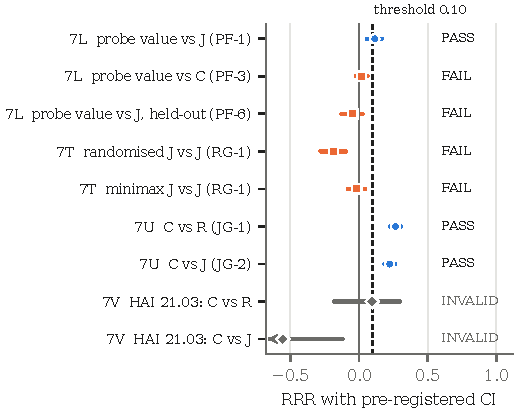
\includegraphics[width=\columnwidth]{figures/fig_forest.pdf}
\caption{Primary contrasts of all four experiments: RRR (marker) and pre-registered interval (bar) against the 0.10
threshold. ``PASS''/``FAIL'' is the gate on that row; E1 passed its headline gate but failed three others and was
killed (Table~\ref{tab:exp}). E4 rows are shown for completeness; the run was invalid. Bars below $-0.65$ are
truncated (arrow).}
\label{fig:forest}
\end{figure}

\begin{table}[t]
\centering
\caption{Primary contrasts. RRR [interval]: 95\% for E1, E3, E4; 97.5\% for E2. ``Pooled families'' are the three E1
attacker families (cover-up, misattribution, trust-harvest).}
\label{tab:primary}
\scriptsize
\setlength{\tabcolsep}{2pt}
\begin{tabular}{@{}lllll@{}}
\toprule
 & Contrast & Gate & RRR [interval] & Result \\
\midrule
\tabinput tables/tab_primary.tex
\bottomrule
\end{tabular}
\end{table}

\subsection{Negative results}\label{sec:neg}

\textbf{E1: decision-valued probing.} $P$ beat $J$ on the pooled attacker families (RRR $\numLJ$ [$\numLJlo$,
$\numLJhi$]), but the experiment was killed by three gates. Against $C$, which uses the same joint model with plain
$H$-information, the gain vanished ($\numLC$ [$\numLClo$, $\numLChi$]). On the held-out misattribution attacker it was
negative ($\numLJmis$ [$\numLJmislo$, $\numLJmishi$]). The pooled gain came from the design attacker, whose behaviour
matches the defender's compromised-source model ($\numLJcov$ [$\numLJcovlo$, $\numLJcovhi$]). Probing was also
untargeted: only about a third of $P$'s probes went to sources the posterior considered suspicious, against a
pre-registered floor of one half.

\textbf{E2: robust acquisition.} E1's exploratory data suggested that model-based policies fail when the attacker does
not match their model. E2 tested two fixes, each changing $J$ in one way: sampling actions in proportion to their score,
and scoring by the worst case over three compromised-source models. On a new held-out attacker neither beat $J$:
randomisation lost clearly ($\numTR$ [$\numTRlo$, $\numTRhi$]) and the minimax policy tied ($\numTM$ [$\numTMlo$,
$\numTMhi$]) while losing on the known families. Both wrappers were built on $J$, the comparator E1 had named; robust
versions of $C$ were not tested.

\subsection{Scoped positive result}\label{sec:pos}

\textbf{Origin, disclosed.} In exploratory tables after the E1 and E2 verdicts, $C$ had lower regret than the one-step
reliability-weighted policy (by 28\% over E1's attacker cells and 55\% on E2's held-out attacker) and than $J$ (by 52\%
on E2's held-out attacker), with near-zero gain against misattribution and trust-harvest. E3 tested this prospectively
against the stricter two-step $R$, on new world seeds and a new held-out attacker (collude-cheap) written before any E3
run. No policy, threshold or world parameter was changed.

\textbf{E3: joint belief.} Every gate passed. On collude-cheap, $C$ reduced regret by $\numUR$ [$\numURlo$,
$\numURhi$] relative to $R$ (Cliff's $\delta=\numcdR$) and by $\numUJ$ [$\numUJlo$, $\numUJhi$] relative to $J$
($\delta=\numcdJ$), with a positive RRR in each attacker budget and in both halves of the worlds, and lower regret than
$R$ on clean worlds. The two contrasts say different things. Against $R$, which shares the objective, horizon, cost
handling, posterior, decision and spend, the gain comes from the look-ahead model, as the package of four differences
listed in Sec.~\ref{sec:model}. Against $J$, which shares the model, the gain comes from the objective: $J$ spends budget
on resolving source states that do not change the decision, and loses to $C$ even on clean worlds ($\numUJclean$
[$\numUJcleanlo$, $\numUJcleanhi$]), so it is a weak reference rather than a strong competitor.

\begin{figure}[t]
\centering
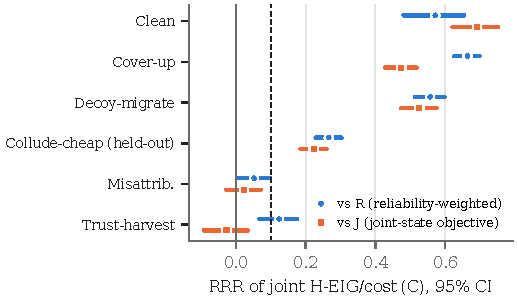
\includegraphics[width=\columnwidth]{figures/fig_scope.pdf}
\caption{E3 scope map (descriptive, not gated): RRR of $C$ against $R$ (circles) and $J$ (squares) by attacker family,
95\% interval. The gain is large against cover-up, decoy and colluding attackers, small against misattribution; against
trust-harvest it remains relative to $R$ but not to $J$.}
\label{fig:scope}
\end{figure}

\textbf{Where it stops.} Fig.~\ref{fig:scope} and Table~\ref{tab:regret} show the limits, which travel with the claim.
(i) The gain tracks how closely the attacker's lies match the defender's model: largest for cover-up, then decoy, then
collude-cheap (half of whose lies are cover-ups), small for misattribution ($\numURmis$ [$\numURmislo$, $\numURmishi$]
relative to $R$). (ii) Against the adaptive trust-harvest attacker, $C$ still beats $R$ ($\numURth$ [$\numURthlo$,
$\numURthhi$]) but not $J$ ($\numUJth$ [$\numUJthlo$, $\numUJthhi$]), and every deterministic policy loses to random
acquisition (regret $\numthRandU$). The same held in E1 (random $\numthRandL$) and E2, where the score-proportional
randomised $J$ ($\numthRandJT$) and uniform random ($\numthRandT$) were the two best. (iii) $C$ is not the best policy on
collude-cheap: nominal EIG, which ignores cost, avoids the cheap sources the attacker controls and does better. The
pre-registered claim is a comparison among cost-aware policies, not ``best against this attacker''.

\begin{table}[t]
\centering
\caption{E3 mean normalised regret by attacker family (\numnWU\ worlds; \numnEU\ policy-episodes in total). Bold:
lowest in the column among all seven policies (one-step $\hat r$ policy not shown).}
\label{tab:regret}
\footnotesize
\setlength{\tabcolsep}{2pt}
\begin{tabular}{@{}lcccccc@{}}
\toprule
Policy & Clean & Cover & Decoy & Collude & Misattr. & Harvest \\
\midrule
\tabinput tables/tab_regret7u.tex
\bottomrule
\end{tabular}
\end{table}

% ---------------------------------------------------------------------------
\section{Real-Data Attempt: HAI}\label{sec:hai}

\textbf{Mapping.} HAI is a public hardware-in-the-loop industrial-control dataset with labelled attacks
\cite{shin2020hai,shin2021hai}; several of its scenarios hold a process variable at a stale value while the process
moves, a real cover-up. We used HAI 20.07 for development (detectors and model fitting, \numVndev\ episodes), HAI 21.03
for the verdict and HAI 22.04 as secondary (nine attacks whose targets the dataset manual leaves ambiguous were
excluded before the run). An episode is one attack segment or a sampled normal window, as many normal windows as
attacks, which sets the base rate at one half by design. Hypotheses are normal, attack confined to the boiler process,
or attack touching the other processes; the three decisions keep their simulator meaning. Nine process variables and
controller outputs are sources. A query reads a source's change alarm over a 30-second window (threshold at the 99th
percentile of attack-free training data). A spoofed variable stays quiet, so the alarm cannot see the spoof itself, only
its absence while other sources move. A probe checks the source against a ridge regression on the other points of its
process. The $k$-th read of a source returns the $k$-th window, up to six reads. The defender model was fitted on
development episodes only and applied unchanged; the protocol was committed before any confirmatory episode was built,
and an in-sample look at the development data was disclosed in it.

\textbf{Outcome: invalid.} V-real failed. On 21.03 nominal EIG improved on the prior-only decision by $\numVoneA$
[$\numVoneloA$, $\numVonehiA$] (\numVnA\ episodes, \numVattA\ attacks, \numVspA\ with spoofing); on 22.04 every
evidence-reading policy did worse than the prior ($\numVoneB$ [$\numVoneloB$, $\numVonehiB$]). Under the pre-registered
rule an invalid run decides nothing, so the comparison of belief models is untested. Table~\ref{tab:hai} shows why the
evidence was too weak: missed boiler attacks dominate regret, and no deterministic policy ever probed (the development
probe failed $\numVfailh$ of healthy and $\numVfails$ of spoofed readings, at twice a query's cost). E4 therefore tested
our detector more than our acquisition rules.

\textbf{Exploratory observations.} Had V-real passed, the E3 replication would have been killed: on 21.03 $J$ had lower
regret than $C$ ($\numVJA$ [$\numVJloA$, $\numVJhiA$]), while on 22.04 the two were level ($\numVJB$ [$\numVJloB$,
$\numVJhiB$]). On 21.03 the lowest regret came from $P$ ($\numVPA$), which never probed and so acted as a
decision-value query selector; this neither revives E1, whose kill concerned probing, nor can be read as evidence under
an invalid run. We do not re-run E4; a new attempt needs a new protocol and evidence that passes V-real first.

\begin{table}[t]
\centering
\caption{E4 (HAI) mean normalised regret, all episodes. V-real compares nominal EIG with the prior-only decision.}
\label{tab:hai}
\footnotesize
\begin{tabular}{@{}lcc@{}}
\toprule
Policy & HAI 21.03 & HAI 22.04 \\
\midrule
\tabinput tables/tab_hai.tex
\bottomrule
\end{tabular}
\end{table}

% ---------------------------------------------------------------------------
\section{Threats to Validity}\label{sec:threats}

\textbf{External validity.} E1--E3 use one simulator family and one world distribution with wide, uncalibrated ranges;
compromise priors up to 0.40 and up to three controlled sources are far above typical tampering prevalence. Sources are
conditionally independent, while real telemetry shares failure modes. The only real-data attempt was invalid, and its
exploratory direction on 21.03 disagreed with E3. The positive result must be read as simulator-only.

\textbf{Model match.} Every attacker, held-out ones included, appears under benign activity with the probability the
defender's coupling assumes, and collude-cheap's lies are half cover-ups. ``Held out'' therefore does not mean
``model-mismatched''. The gain of $C$ shrinks as the match weakens (Sec.~\ref{sec:pos}), and the same researcher wrote
the policies and the attackers.

\textbf{Attribution.} The $C$-vs-$R$ gain belongs to a package of four modelling differences, not one; the
$C$-vs-$J$ gain is an objective effect against a comparator that is weak even on clean worlds. Separating the four model
differences, testing a joint model with a deliberately wrong compromise likelihood, and varying the assumed forge rate
are needed before naming a mechanism.

\textbf{Missing comparators.} We did not test longer-horizon or POMDP planners, Thompson sampling or
expected-error-reduction rules, cost-aware nominal EIG in E3, or robust wrappers around $C$.

\textbf{Exploratory origin.} E3's hypothesis came from E1 and E2 data after their verdicts. E3 is its first prospective
test; a second independent test has not been done.

\textbf{Construct validity.} Regret is normalised per world and RRR is a ratio of sums, so worlds with large regret
weigh more; per-budget, per-half results and Cliff's $\delta$ are reported to show the effect is not driven by a few
worlds. The HAI mapping (change alarms, a regression probe, three coarse hypotheses, balanced base rate) is one of many
possible and was too weak.

\textbf{Multiplicity.} Each experiment controls its own error rate (intersection--union across comparators; Bonferroni
across E2's two candidates). Across the four experiments we report every outcome, including the failures.

% ---------------------------------------------------------------------------
\section{Conclusion}

Among cost-aware Bayesian acquisition rules in our simulator, the parts that mattered were the look-ahead model and the
objective: modelling each source's compromise state jointly with the hypothesis, and spending budget on information
about the hypothesis rather than about the sources. That result holds against attackers whose lies resemble the
defender's model, shrinks against misattribution, and against an attacker that exploits the defender's choices it
survives only relative to reliability weighting, while random acquisition is best. It is not yet supported by real data,
and the one real-data look, though invalid, pointed the other way on the objective contrast. Decision-valued probing and
robust wrappers both failed pre-registered tests; of the three ideas tested in simulation, two failed.

\textbf{Practical implications.} Two cautious lessons follow. First, if a source can be compromised, model how it would
lie rather than down-weighting it as noise, and judge evidence by what it says about the incident rather than about the
sources. Second, when an attacker can watch which sources the hunter relies on, a fixed, model-driven reading order is
exploitable; in every simulated experiment, randomising the order did better against such an attacker. Neither lesson
replaces calibrated per-source models, which a SOC rarely has.

\section*{Artifact Availability}
Code, protocols, gate code, raw outputs, statistics and verdicts are in the repository
\url{https://github.com/ftaakash/Hades} (branch \texttt{claude/hades2-probe-pilot-gemc0j}). Experiment IDs:
E1 \texttt{phase7l\_probe\_pilot\_v2}, E2 \texttt{phase7t\_robust\_pilot\_v1}, E3 \texttt{phase7u\_joint\_belief\_v1},
E4 \texttt{phase7v\_hai\_replication\_v1}. Every number in this paper is regenerated from the raw outputs by
\texttt{scripts/paper/recompute\_headlines.py} and \texttt{scripts/paper/make\_figures.py}. HAI is available from
\url{https://github.com/icsdataset/hai} under CC BY-SA 4.0.

\bibliographystyle{IEEEtran}
\bibliography{refs}

\end{document}
